\chapter{计算机组成原理}\label{ch:arch}

被誉为现代计算机之父的冯·诺依曼(Von Neumann)在1945年提出了一种计算机架构,后被称为\textbf{冯·诺依曼架构}。这种架构由\textbf{中央处理器(CPU)}、\textbf{存储器}和\textbf{输入输出设备}三部分组成。本章将逐一介绍这三大部分的作用以及它们之间的运作模式。


\section{存储器}\label{sec:arch:storage}

在计算机的世界里,一切的内容(文本、图像、音频、视频等)都被称为\textbf{数据}。在\textbf{二进制计算机}中,数据是由$0$和$1$组成的字符串,被称为\textbf{比特流}。比如在Unicode字符集中,“你好世界”四个字符被分别表示为以下比特流:

\begin{center}
    %! suppress = EnDash
    \begin{tabular}{ c c c }
        \hline
        字符 & Unicode & 比特流                        \\
        \hline
        你  & U+4F60  & 11100100 10111101 10100000 \\
        好  & U+597D  & 11100101 10010111 10111101 \\
        世  & U+4E16  & 01001110 00010110          \\
        界  & U+754C  & 0111010101001100           \\
        \hline
    \end{tabular}
\end{center}

用于表示图像和视频的方式很复杂,对应的比特流也非常长。这些数据被计算机处理后通过数据线传输到显示器,显示器再将这些数据显示出来,使我们能够在屏幕上看见缤纷多彩的图画。正如水要装在瓶子里,书要放在书架上,数据也需一个安身之处。而\textbf{存储器}就是数据的家。

存储器是用于\textit{存储数据的记忆部件}。其有两种类型,分为是主存储器(通常称为\textbf{内存}或\textbf{运行内存})和辅助存储器(通常称为\textbf{外存}或\textbf{内部存储})。二者最大的区别在于,\textit{内存是断电即失的,而外存一旦被写入,数据便不会消失}。在计算机运行时,数据会暂时被安放在内存中;而当我们保存文件时,数据则会被写入到外存中。如果未保存文件时计算机突然断电,那么数据就会丢失且无法被找回。

将数据存入存储器中的过程称为\textbf{写入};将数据从存储器中取出的过程称为\textbf{读取}。读取和写入统称为\textbf{读写}。大部分存储器都支持读写,但一些存储器,如光盘(CD和DVD)和磁带,则是\textbf{只读}的。

一台完整的现代计算机,如手机和笔记本电脑,在出厂时就会内置一个内存和一个存储器。由于这些部件被包裹在金属和塑料外壳内,一般人很少会接触到。但是\textbf{移动存储器}在生活中确十分常见,如U盘、移动硬盘以及上文提到的光盘和磁带等。这些存储器一般通过\textbf{接口}与计算机连接并传输数据。而光盘和磁带这种形状特别的存储器,需要特制的驱动器读取数据。如光盘必须放入\textbf{光盘驱动器}(简称\textbf{光驱})中,而磁带则必须放入\textbf{磁带驱动器}(简称\textbf{磁带机})中。

存储器大小各异。在手机上,一张拇指大小的\textbf{SD卡}就可以存储512GB的数据;在电脑上,一个巴掌大小的固态硬盘(又称\textbf{SSD})的存储大小可能也就翻一倍。然而,虽然\textbf{存储容量}相差无几,体积大的存储器一般\textbf{读写速度}更快。此外,在市场上,\textit{读写速度越快、存储容量越大的存储器,价格越贵}。


\section{中央处理器}\label{sec:arch:cpu}

计算机之所以被称为计算机,就是因为它的主要职责就是计算。说得难听点,它就是\textit{一台只会计算四则运算(加减乘除)的机器}。\textbf{中央处理器}(简称\textbf{CPU})是计算机中负责计算的元件。其通过\textbf{控制模块}将内存中的数据读入到\textbf{寄存器}中,经过计算后,将结果重新写入到内存中。

在深入探讨中央处理器之前,我们先来设想一个现实生活中的例子。餐厅的后厨有一位厨师,一位学徒,和一个冰箱。学徒需要从冰箱中取出食材,装到一个篮子里,送到厨师手上;厨师对食材进行加工(烹饪),随后将菜品呈递给学徒;学徒再将菜肴端送给顾客。注意:这位厨师非常有架子,他不会主动去冰箱获取食材,只会吆喝他的学徒给他递送食材。其次,这个冰箱十分神奇,学徒从冰箱中拿出食材时,冰箱会复制一份食材让学徒取用,而原先的食材不会发生变化。

有了上述例子,我们就可以理解CPU,内存和硬盘(外存)之间的关系了。CPU(厨师)只会处理内存(学徒)中的数据(食材),并将处理后的数据存回到内存中。CPU不能直接访问外存(冰箱),任何外存中的数据都必须先加载到内存中,才能被计算。比如,我们想要使用微信,必须先从软件市场\textbf{下载}到手机上。我们会在之后的章节讨论\textbf{下载},但其最终结果是:手机的\textbf{外存}中多出一个叫\app{微信}的软件。当我们打开\app{微信}时,手机需要先把\app{微信}这个软件从外存复制到内存中。这个过程称为\textbf{加载}(或\textbf{载入})。在我们成功进入\app{微信}时,整个程序就已经加载完毕了,并且每当我们执行一个操作(如发送消息、进入朋友圈等),\app{微信}都要将数据传到CPU中进行计算,得到新的结果后,软件的状态会被更新,而我们便会看到屏幕上显示的内容发生变化。图\ref{fig:cpu_memory_storage}展示了CPU、内存和硬盘之间的关系。

\begin{figure}[htbp]
    \centering
    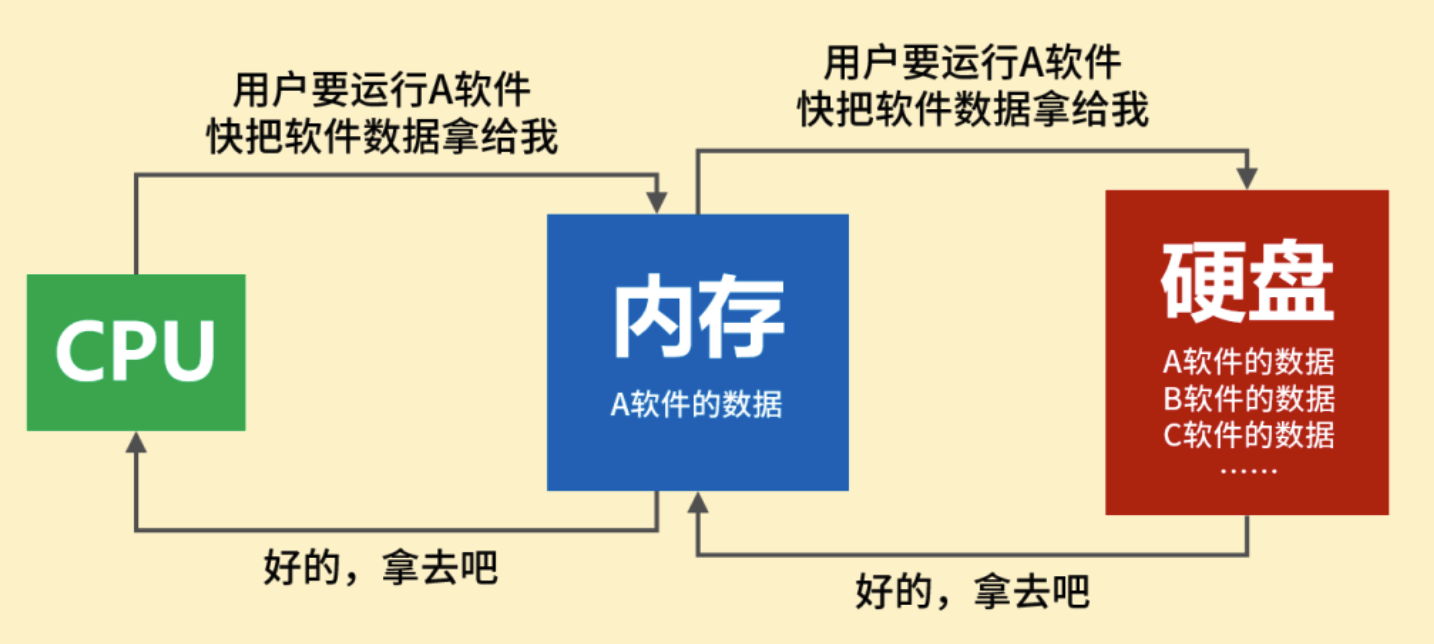
\includegraphics[width=0.75\textwidth]{images/ch2/cpu_memory_storage}
    \caption{
        CPU只能与内存交互;内存可以从硬盘中拷贝数据,并让CPU处理。
    }
    \label{fig:cpu_memory_storage}
\end{figure}


\section{输入输出设备}\label{sec:arch:io_devices}

除了CPU和内存,其他所有的设备都是输入输出设备(简称IO设备),如屏幕、按钮、扬声器、麦克风等。我们对常见的输入输出设备进行分类:

\begin{itemize}
    \item {
        \textbf{输入设备}: 键盘,鼠标,功能按钮,麦克风,触摸屏,信号接收器,光驱等。
    }
    \item {
        \textbf{输出设备}: 显示器(屏幕),扬声器,音响,有线耳机,打印机等。
    }
\end{itemize}

不难发现,输入设备向计算机内存传输数据。拿键盘举例:每当我们按下一个按键时,这个事件相关的数据就会传入到计算机内存的特定区域(称为\textbf{缓冲区});操作系统随后可以读取这些数据,并进行一系列的处理。输出设备则接收计算机内存中的数据,并通过各种方式呈现给使用者。如麦克风会将数据转化为声音并播放出来;显示器会将数据转化为特定的图像并显示出来。

值得注意的是,触屏手机的屏幕包含一个输入设备和一个输出设备:触摸屏(一块透明的玻璃)是输入设备;显示屏是输出设备。这两个设备紧密地粘接在一起,就好像只有一块薄薄的屏幕一样。有时我们会发现屏幕明明可以正常地显示图像,但却怎么点手机都没有反应。这是因为显示屏完好无损,但透明的触摸板损坏或接触不良,导致我们的滑动和点击操作无法被转换为特定的数据存入内存中。

在家用计算机(如手机,电脑,电视等)中,显示器是最重要的输出设备。我们来探讨显示器如何输出图像到显示器上。当凑近屏幕时,我们会发现屏幕实际上是由很多极其细小的“灯”组成的。这些灯排列为一个$1920 \times 1080$(注:分辨率更高的显示器,灯的个数更多)的方阵。每个“灯”可以发出三种颜色的光:红、绿、蓝。假设所有的灯都同时亮起三种颜色的光,那么当我们离屏幕较远时,这些光会合成若干道白光进入我们的眼睛。而如果所有的灯亮起蓝光,而没有亮起红光和绿光,那么我们就会看到一个完全蓝色的屏幕。软件通过控制内存中的数据,就能控制每盏灯所亮的光,就能准确地显示各种各样的画面。软件可以通过快速的改变内存中的数据,使得屏幕的画面快速变化。传入到我们的眼中,便是一连串快速变化的图像,也就是人们常说的\textbf{视频}。


\section{电源}\label{sec:arch:battery}

众所周知,计算机是电器,也是人们进入电气时代后最伟大的发明之一。电器当然离不开电咯。每个计算机中都有一个\textbf{电源}设备,它为CPU、内存和输入输出设备提供充足的电量。我们一般不认为电源是输入输出设备,但非要说的话,手机中的电池属于输出设备,因为它每时每刻都向内存写入它的剩余电量等信息。

如今,绝大多数\textbf{可移动设备}(手机、平板电脑、笔记本电脑、智能手表、蓝牙耳机等)所用的电池都是\textbf{锂电池}。锂电池具有\textbf{寿命}。每当它放电时,它的寿命就会减少,具体表现为“用得更快”。一个锂电池用了5年后,它的电池寿命就会降低一半。也就是说,手机充满电后,只能支撑相当于出厂时一半的待机时间。所以,我们可以每隔三四年去找售后换一个新的手机电池,或者买一台新的手机。现在的绝大多数可移动设备在充电时,都不会消耗电池电量,而是直接消耗外部输入的电量。因此不再会出现“边充电变用手机导致电池寿命锐减”的现象。

在计算机中,CPU是消耗电量的主要原件。\textbf{计算任务越繁重,电量的消耗速度越快}。在上一节中我们提到过,显示器播放视频的原理就是快速地切换图像。这个过程需要大量的计算(因为计算机内部要计算 $1920 \times 1080$个像素点的状态,即“发什么光”)。因此,看视频和玩游戏都十分消耗电。除此之外,启用无线网络和蓝牙也会消耗大量电量。我们若想省电,可以关闭Wi-Fi和蓝牙,并打开“飞行模式”(注:打开飞行模式后,我们无法接收一切移动数据,包括电话和短信)。


\section{接口和数据线}\label{sec:arch:interfaces_cables}

计算机中,各个设备间需要相互传输数据。输入输出设备分为\textbf{内部设备}(被包裹在设备中的原件)和\textbf{外部设备}。比如,麦克风和扬声器是手机的内部设备,而键盘和鼠标则是外部设备。内部设备在手机壳里通过细小的电线(或电路板上的电路)与内存、CPU交换数据。而外部设备则需要通过\textbf{接口}实现这一点。接口按用途可分为:

\begin{enumerate}
    \item { \textbf{数据接口}: 用于交换数据的接口 }
    \item { \textbf{充电器接口}: 用于为设备和电池提供外部电源的接口 }
    \item { \textbf{(数据电源)一体化接口}: 为了方便用户使用,现在大部分移动设备都提供了一体化接口。这类接口既可以交换数据,也可以为设备充电 }
\end{enumerate}

\begin{figure}[htbp]
    \centering
    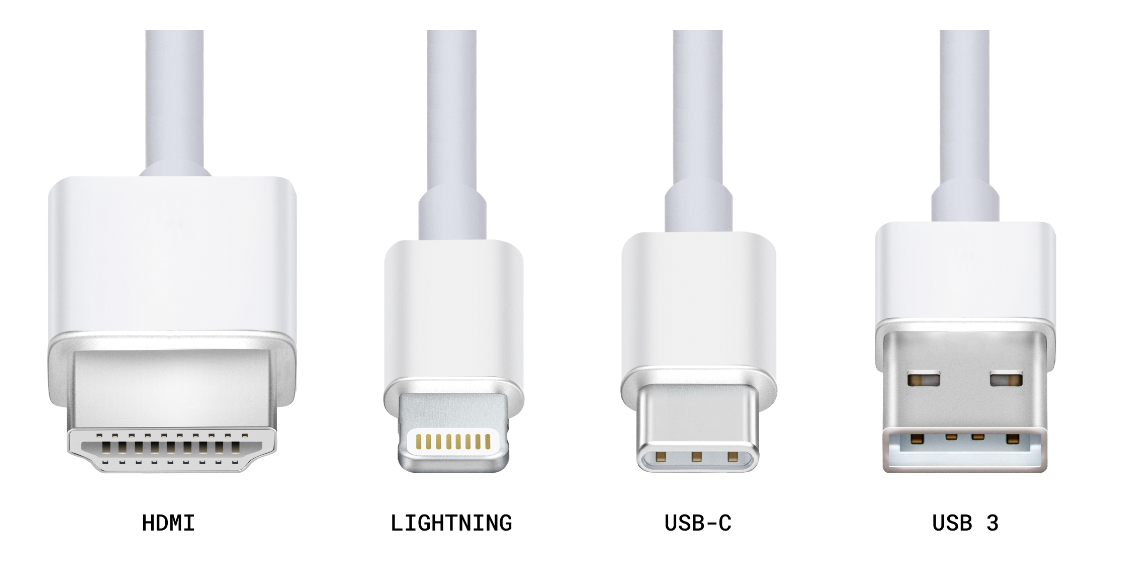
\includegraphics[width=0.75\textwidth]{images/ch2/four_interfaces}
    \caption{
        四种不同的接口,从左到右分别为:HDMI、Lightning、USB-C 和 USB3
    }
    \label{fig:cpu_four_interfaces}
\end{figure}

接口按型号分可以分为(见图\ref{fig:cpu_four_interfaces}):

\begin{enumerate}
    \item { \textbf{USB接口}: 用于传输数据和充放电 }
    \item { \textbf{USB-C(或Type-C)接口}: 新一代USB接口,用于传输和充放电,并逐步替代USB接口 }
    \item { \textbf{HDMI接口}: 用于传输高清视频数据,常见于显示器 }
    \item { \textbf{Lightning接口}: 苹果设备的旧接口,现已淘汰 }
    \item { ......(还有很多其它接口,但都不常用,我们就不一一学习了) }
\end{enumerate}

假如我们有一天买回来了一个机顶盒和一台电视机,我想让\textbf{机顶盒}(如DVD机)的画面数据传输到电视机上并显示,该怎么安装呢?注意到此处的“电视机”可以被视为一台显示器,或者说一个外部输出设备。我们首先为两个设备接通电源,然后使用一条数据线连接两台设备。数据线的一端接入电视机的HDMI接口,另一端接入机顶盒的HDMI接口。接入完成后,在电视机中切换到与接入口相匹配的频道,即可显示机顶盒中的画面数据。


\section{习题}\label{sec:arch:exercise}

\multiplechoice{
    1. 以下哪个选项不属于冯·诺依曼计算机架构?
} {
    存储器,
    显示器,
    中央处理器(CPU),
    输入输出设备
}

\multiplechoice{
    2. 以下说法不正确的是
} {
    在手机上,内部存储简称内存,
    DVD需要光驱才能读取,
    将U盘插入计算机上相应的接口,一切正常的话,计算机可以对U盘进行读写,
    在计算机中,视频与文本都以比特流的方式存储在存储器中
}

\multiplechoice{
    3. 以下存储器支持读写的是(多选)
} {
    CD,
    U盘,
    磁带,
    移动硬盘
}

\multiplechoice{
    4. 以下说法正确的是(多选)
} {
    CPU可以直接访问U盘,
    在打开\app{美团}时,外存中的\app{美团}APP被完整地复制到内存中后,我们才能使用,
    CPU只是用来计算的,它不能存储大批量的数据,
    CPU计算后的结果,可以被重新存放至内存中
}

\multiplechoice{
    5. 以下是输出设备的设备有(多选)
} {
    显示器,
    音响,
    有线鼠标,
    DVD光驱
}

\multiplechoice{
    6. 以下关于电源说法正确的是
} {
    边充电边用手机会加速手机电池的损耗,
    锂电池会随着放电时间的增加而减少寿命,变得越来越不耐用,
    台式计算机需要外接电源,故无需安装电池,
    电池的消耗速度与计算机当前的计算压力无关
}

\openEnded{
    7. 小明很不解:“真是无语了。为什么我待机听歌很长时间电量都没怎么减少,而打游戏的时候电量一下就见底了啊?”请用你所学的知识帮他解答他的疑问吧!
}

\openEnded{
    8. 欧洲理事会于2022年10月24日批准了“在欧盟范围内统一充电器接口”的法案,在2024 年底之前,USB Type-C接口将成为一系列电子设备的通用充电标准。想一想:接口为我们提供了哪些便利?为什么我们应当推进“接口统一”的进程。
}